\section {Best Ever Alarm System Toolkit - BEAST}

\subsection {Introdução} \label{beast-intro}

Em um ambiente composto por centenas de milhares de variáveis EPICS, como o que
será implementado no \textit{Sirius}, a necessidade de um sistema capaz de
monitorar quais variáveis encontram-se em estados errôneos torna-se
imprescindível. Sendo assim, o monitor de alarmes \textit{BEAST}, do inglês
\textit{Best Ever Alarm System Toolkit} e desenvolvido pelo laboratório
americano \textit{Oak Ridge National Laboratory}, representa uma solução capaz
de gerenciar e controlar os alarmes gerados pelos servidores EPICS disponíveis
na rede. Tal sistema é implementado em \textit{Java} e é baseado no ambiente
gráfico de desenvolvimento \textit{Eclipse}. A arquitetura do sistema
está represetada na figura \ref{fig:best_arquitetura}, logo abaixo.

\begin{figure}[h]

\centering
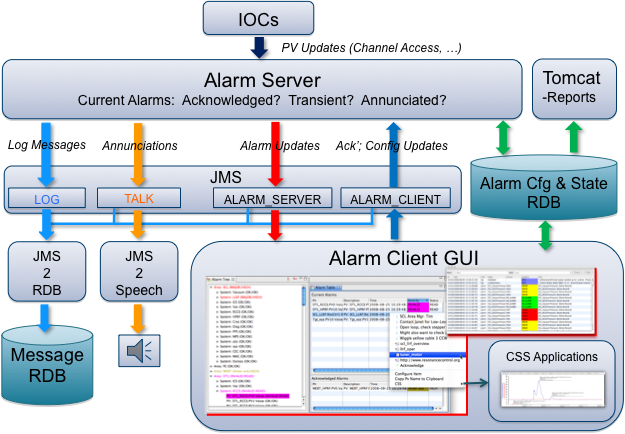
\includegraphics[scale=0.40]{image/beast-arquitetura}
\caption {Implementação do sistema de monitoramento de alarmes
\textit{BEAST}. Extraída de \cite{beast}.}
\label{fig:best_arquitetura}
\end{figure}

É possível distinguir diversos componentes na figura acima:

\begin{enumerate}[i.]
  
  \item \textit{Alarm server}: o servidor é responsável por tarefas fundamentais
  no monitoramento de alarmes. Cabe a ele a leitura da configuração dos alarmes
  armazenada no banco de dados \textit{Alarm Cfg \& State RDB}, conectar-se às
  respectivas variávies, monitorar suas mudanças de estado e gerar alarmes
  quando necessário e desativá-los logo que um operador toma conhecimento
  do problema. Esse módulo permite que um número variável de clientes se conecte
  a ele. Uma variável pode adotar duas configurações distintas, sendo elas
  \textit{latch} e \textit{annunciate}. Para a primeira, o servidor mantém o
  alarme de maior gravidade, mesmo que o estado da variável não seja
  atualmente errôneo, até que ele seja reconhecido manualmente pelo operador.
  A fim de impedir um grande volume de alarmes gerados, é possível habilitar
  as opções \textit{delay}, que aciona o alarme somente se o estado errôneo da
  variável se mantiver durante o intervalo de tempo especificado, e
  \textit{count}, que aciona o alarme se tal estado for detectado mais vezes
  que o valor especificado. A segunda configuração ativa o alarme somente
  quando a \textit{PV} apresentar valor inválido, sendo que ele é desativado
  logo que tal variável voltar à sua faixa de operação esperada.
  
  \item \textit{Alarm Cfg \& State RDB}: banco de dados relacional, como um
  servidor \textit{MySQL} por exemplo, onde serão armazenadas as configurações
  de alarme e o atual estado de todos os alarmes.
  
  \item \textit{Java Message Service - JMS}: utilizado para a comunicação entre
  diferentes módulos. No projeto, foi empregada a implementação realizada pelo
  \textit{Apache Software Foundation} chamada de  \textit{Apache ActiveMQ}. O
  sistema utiliza 4 \textit{topics} distintos, sendo eles:
  
  \begin{itemize} \renewcommand\labelitemi{--}
    \item \textit{ALARM\_SERVER}: utilizado pelo servidor para publicar
    atualizações nos estados dos alarmes de acordo com a configuração de cada
    variável.
    
    \item \textit{ALARM\_CLIENT}: permite que clientes notifiquem atualizações
    de configuração e reconhecimento de alarmes.
    
    \item \textit{TALK}: dedicado para anunciar mensagens.
    
  \end{itemize}
  
  \item \textit{Alarm Client GUI}: \label{client-gui} baseado na interface
  gráfica do \textit{Eclipse}, oferece três opções de monitoramento:
  
  \begin{itemize} \renewcommand\labelitemi{--}
    \item \textit{Alarm table}: mostra os alarmes em duas tabelas distintas
    contendo aqueles reconhecidos (\textit{acknowledged alarms}) e aqueles que
    ainda estão acionados (\textit{active alarms}).
    
    \item \textit{Alarm tree}: essa opção de visualização oferece
    uma visão hierárquica dos alarmes, sendo organizada, do nível mais alto para
    o menor, em áreas, sistemas, subsistemas e variáveis. Oferece opções para
    configurar, remover ou adicionar variáveis no nível desejado. O estado do
    alarme de cada item é mostrado por uma cor e por uma anotação, sendo
    composta por três sentenças entre parênteses, que representam
    respectivamente a gravidade atual (\textit{current severity}), a
    maior gravidade detectada anteriormente (\textit{alarm severity}) e o estado
    atual do alarme (\textit{alarm status}). É sincronizada diretamente ao banco
    \textit{Alarm Cfg \& State RDB}, o que implica que uma mudança realizada é
    rapidamente detectada pelo servidor e pelos demais clientes.
    
    \item \textit{Alarm area panel}: indicação gráfica do estado do sistema.
    
  \end{itemize}
  
  É possível, a partir de qualquer uma das \textit{views} presentadas acima,
  acessar outros recursos, como, por exemplo, gráficos e valores atuais das
  variáveis desejadas. Para isso, basta apertar com o botão direito acima da
  \textit{PV} e apertar em \textit{Process variables}. A implementação fornece,
  ainda, suporte para autenticação de usuários via \textit{LDAP} ou
  \textit{JAAS}. Caso seja a escolha, somente usuários autorizados podem alterar
  as configurações de alarmes ou reconhecê-los.
  
\end{enumerate}

\subsection{Instalação}

\textit{BEAST} necessita de uma base de dados relacional, de uma implementação
\textit{JMS} e de uma instalação do \textit{Eclipse} contendo todos os
\textit{plugins} dos quais o servidor de alarmes depende. O último só é
necessário para exportar o produto a partir do código fonte. Depois
de ter sido exportado, a versão do \textit{Eclipse} pode ser
descartada. Utilizamos o \textit{MySQL}, \textit{Apache
ActiveMQ} e a versão \textit{Eclipse Luna for RCP and Plugin Development} para
os requisitos acima. O servidor de alarmes encontra-se no OPR23, assim
como o arquivador.


\subsection{Uso da interface \textit{Eclipse} como \textit{Alarm Client GUI}}

Para utilizar o \textit{Eclipse} como um cliente do servidor de alarmes, é
necessário configurá-lo para que ele acesse os servidores \textit{MySQL} e
\textit{JMS}. Isso é realizado através de \texttt{Window > Preferences > CSS
Applications > Alarm > Alarm System}. Se tudo foi configurado corretamente, já é
possível acessar os alarmes configurados através do componentes comentados no
item \ref{client-gui} da seção \ref{beast-intro}. A figura \ref{fig:alarm}
representa alguns alarmes que configuramos no grupo de Controle. Destaca-se a
variável \texttt{Cnt:MikroE:GPS:Fix}, criada na seção \ref{sec:pvsgps}.

\begin{figure}[h]
\centering
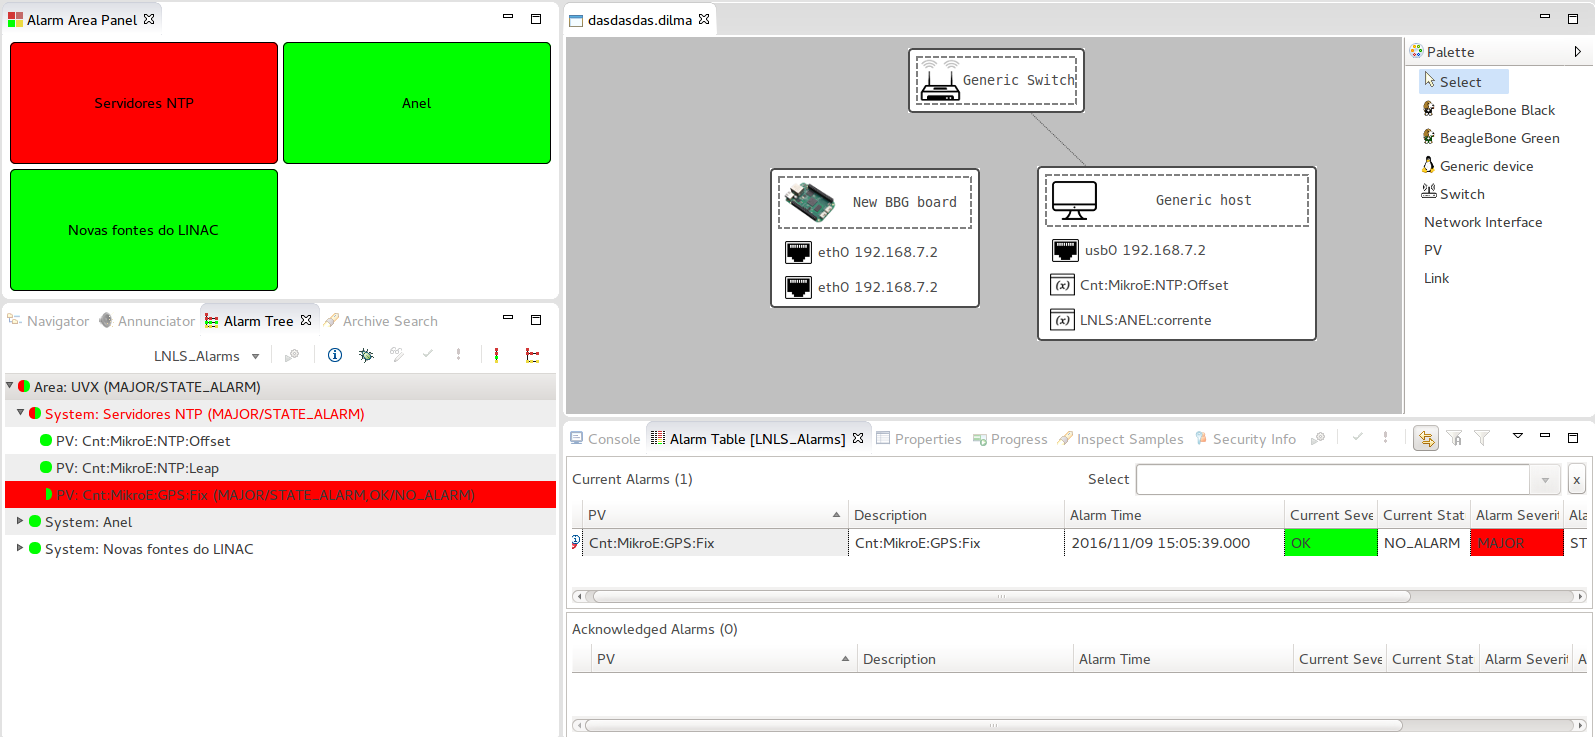
\includegraphics[width=0.95\textwidth]{image/beast-screen-shot}
\caption {Cliente \textit{BEAST} baseado no \textit{Control System Studio}.}
\label{fig:alarm}
\end{figure}

\subsection {Obtendo um \textit{LNLStudio} a partir da configuração do
\textit{Eclipse}}

O \textit{Eclipse} provê suporte para projetos do tipo
\textit{Plugin Project}, específicos para a criação de novos produtos e
\textit{plugins}. Sendo assim, foi possível exportar a configuração atual do
\textit{Eclipse} como um novo produto, que chamaremos de \textit{LNLStudio}.
Isso foi realizado através da seleção de apenas os \textit{plugins} que são
importantes para o grupo, tais como aqueles ligados ao \textit{BEAST} e ao
construtor de interfaces \textit{OPI Builder}.  Em relação a outros produtos
originados do \textit{Control System Studio}, o \textit{LNLStudio} proporciona
uma maior liberdade de configuração e modificação de parâmetros como, por
exemplo, a possibilidade de autenticação a um servidor LDAP. Além disso, o
último \textit{LNLStudio} foi construído a partir da versão 4.1.4 do CSS, sendo
mais recente do que muitos dos demais produtos disponíveis. A figura
\ref{fig:alarm} foi gerada a partir do \textit{LNLStudio}.

 